\documentclass{sigchi}

%\toappear{Copyright\copyright~2015. edX. This document may be redistributed under the terms of the CC-BY-SA 3.0 or later, or AGPL v3.0 or later. See \textsc{https://creativecommons.org/licenses/by-sa/3.0/} and \textsc{http://www.gnu.org/licenses/agpl-3.0.en.html} for details.}

%% EXAMPLE BEGIN -- HOW TO OVERRIDE THE DEFAULT COPYRIGHT STRIP -- (July 22, 2013 - Paul Baumann)
\toappear{ Copyright \copyright 2015. edX. This document may be redistributed under the terms of the CC-BY-SA 3.0 or later, or AGPL v3.0 or later. \\
See: \textsc{https://creativecommons.org/licenses/by-sa/3.0/}\\
\textsc{http://www.gnu.org/licenses/agpl-3.0.en.html} for details.\\
{\emph{UIST'15}}, November 8-11, 2014, Charlotte, NC.}
%% EXAMPLE END -- HOW TO OVERRIDE THE DEFAULT COPYRIGHT STRIP -- (July 22, 2013 - Paul Baumann)


% Arabic page numbers for submission. 
% Remove this line to eliminate page numbers for the camera ready copy
% \pagenumbering{arabic}


% Load basic packages
\usepackage{balance}  % to better equalize the last page
\usepackage{graphics} % for EPS, load graphicx instead
\usepackage{times}    % comment if you want LaTeX's default font
\usepackage{url}      % llt: nicely formatted URLs

% llt: Define a global style for URLs, rather that the default one
\makeatletter
\def\url@leostyle{%
  \@ifundefined{selectfont}{\def\UrlFont{\sf}}{\def\UrlFont{\small\bf\ttfamily}}}
\makeatother
\urlstyle{leo}


% To make various LaTeX processors do the right thing with page size.
\def\pprw{8.5in}
\def\pprh{11in}
\special{papersize=\pprw,\pprh}
\setlength{\paperwidth}{\pprw}
\setlength{\paperheight}{\pprh}
\setlength{\pdfpagewidth}{\pprw}
\setlength{\pdfpageheight}{\pprh}

% Make sure hyperref comes last of your loaded packages, 
% to give it a fighting chance of not being over-written, 
% since its job is to redefine many LaTeX commands.
\usepackage[pdftex]{hyperref}
\hypersetup{
pdftitle={Collaborative Multimodal Annotation System for Peer Discussion at Scale},
pdfauthor={LaTeX},
pdfkeywords={SIGCHI, proceedings, archival format},
bookmarksnumbered,
pdfstartview={FitH},
colorlinks,
citecolor=black,
filecolor=black,
linkcolor=black,
urlcolor=black,
breaklinks=true,
}

% create a shortcut to typeset table headings
\newcommand\tabhead[1]{\small\textbf{#1}}


% End of preamble. Here it comes the document.
\begin{document}

\title{Multimodal Peer Discussion at Scale}

\numberofauthors{3}
\author{
  \alignauthor Dongwook Yoon\\
    \affaddr{Cornell University}\\
    \affaddr{Ithaca, NY 14850}\\
    \email{dy252@cornell.edu}\\
  \alignauthor Piotr Mitros\\
    \affaddr{edX}\\
    \affaddr{Cambridge, MA 02139}\\
    \email{pmitros@edx.org}\\
}

\maketitle

\begin{abstract}
Abstract
\end{abstract}

\keywords{
	Massive open online courses; peer discussion; multimodal annotation; voice user interface; peer group assignment.
}

\category
{H.5.3.} Group and Organization Interfaces: Collaborative computing; {H.5.2.} User Interfaces: Interaction styles; {H.5.1.} Multimedia Information Systems: Audio input/output.

\section{Introduction}

Peer-discussion is an important interactive learning activity that can strengthen students’ mental model about classroom concepts \cite{nicol2003peer} and broaden their perspective on problem solving \cite{smith2009peer}.
Massive open online course providers endeavored to provide a large number of students with online peer discussion activities through discussion forums or video chats.
However, those communication tools does not support both of the rich face-to-face like communication modalities and the flexibility of asynchronous interaction together.

Recently, Yoon et al. presented a multimodal annotation system called RichReview \cite{yoon2014richreview}.
RichReview brought expressivity of multimedia recording into asynchronous document annotations.
Although the original system was built for the writing feedback purpose, we acknowledged the potential of repurposing RichReview's interaction model for supporting online peer-discussion.

In this work, we will demonstrate how integration of RichReview into a MOOC platform can potentially open an expressive discussion channel among a large number of students.
As the first step, we re-implemented the RichReview's front-end as an course applet in the platform of edX--one of the largest MOOC providers.
Then we designed a scalable back-end architecture for transmitting and storing multimedia comments created by a number of students.
And finally, we present a novel peer-group assignment scheme that maximizes overall diversity of group composition using students profile data.

\begin{figure}[!h]
\centering
{
\setlength{\fboxsep}{0pt}
\setlength{\fboxrule}{0.5pt}
\fbox{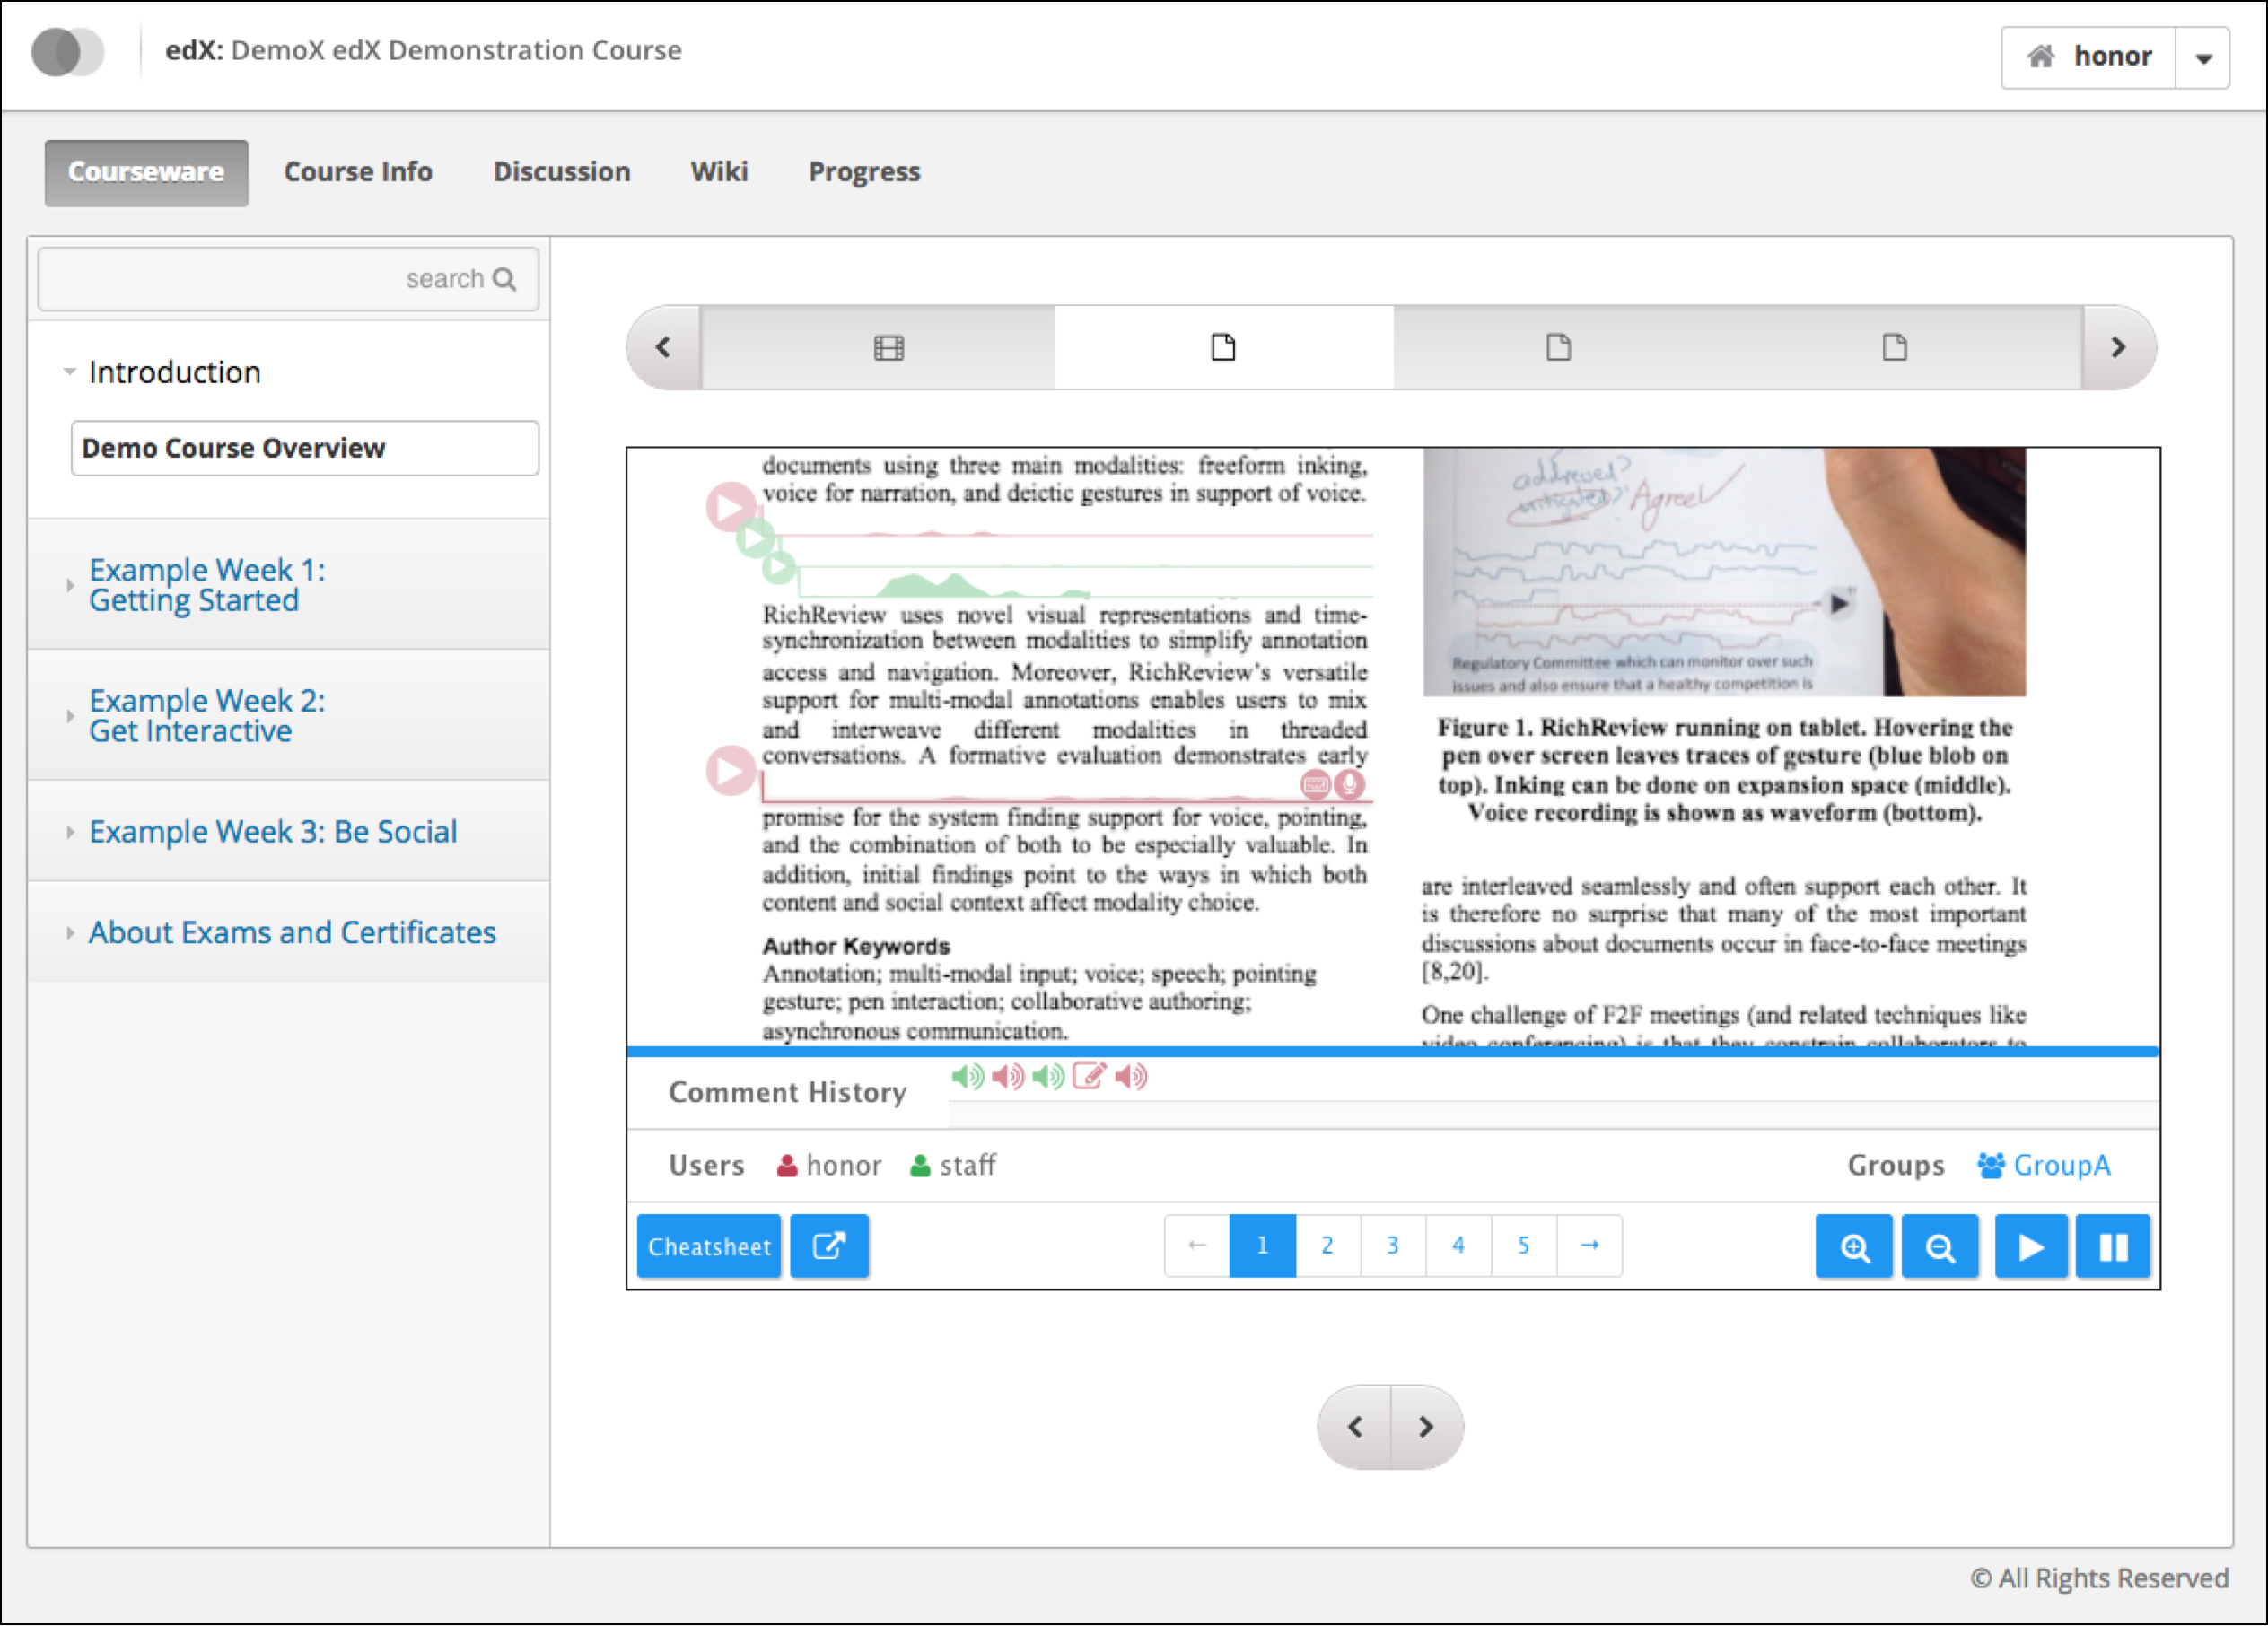
\includegraphics[width=0.95\columnwidth]{figure_edx}}
}
\caption{The RichReview web applet running in the edX courseware.}
\label{fig:figure1}
\end{figure}


\section{Previous Work: RichReview Multimodal Annotation System}
RichReview is a tablet based multimodal annotation system for bringing richness of in-person conversation into document writing revision process.
With RichReview, a commentator can record a combination of input modalities that are available in the modern tablet computers, such as digitizer writing, voice recording, and the pen's hovering.
For example, a RichReview users can verbally explain about a math concept while pointing over a relevant formula and drawing a graph.
Moreover, apart from other anchored discussion systems, RichReview puts an annotation thread within text lines of the body passage, so that the surrounding texts could enrich the context of the comments.
A prior lab study promised potential of the rich commenting system as a supporting tool for document-centric conversation.

\begin{figure}[!h]
\centering
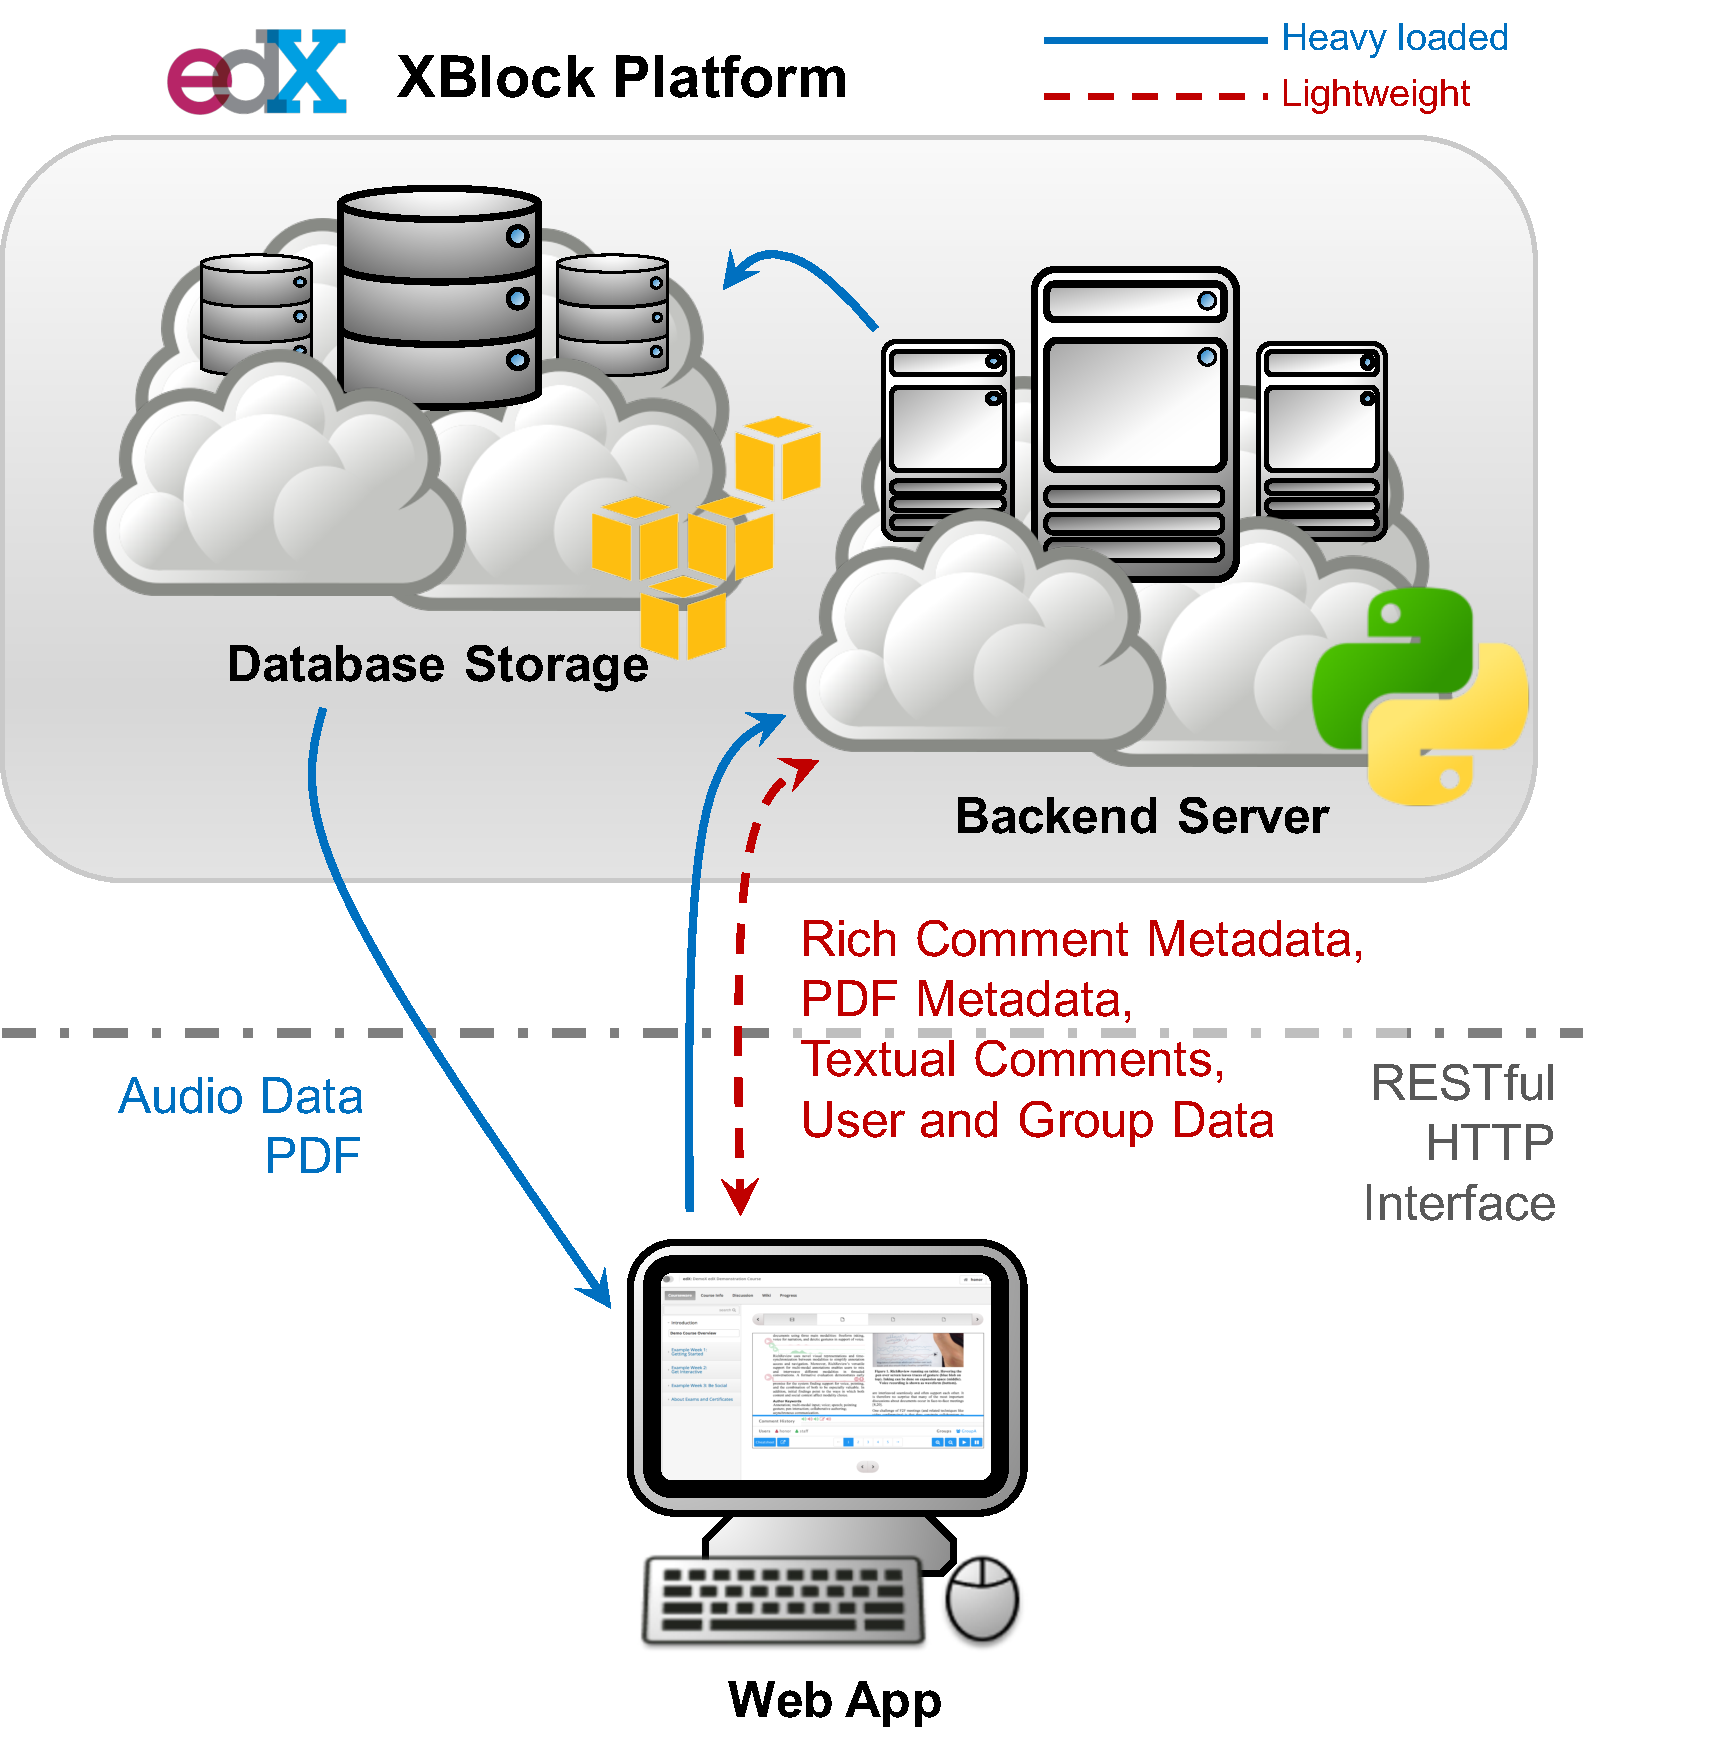
\includegraphics[width=0.95\columnwidth]{figure_architecture}
\caption{Scalable back-end architecture of the multimodal annotation system.}
\label{fig:figure2}
\end{figure}

\section{Integration into edX.org} 

The key to success for the deployment of a courseware application is a seamless integration into the existing MOOC service platform.
As an integral part of the edX.org, we re-implemented the RichReview system as an extension of XBlocks, courseware components for authoring edX courses.
This allows the MOOC authors to include RichReview discussion sessions without having the hassles of the service management.
For example, as shown in the Figure 1, the instructor can place the RichReview discussion session within the flow of the course contents.
Note here that The RichReview XBlock serves the discussion session as an the JavaScript-based web application front-end.

\subsection{Making the Back-end Scalable}
RichReview is a media-heavy web application that frequently exchanges audio-visual data with the server.
Thus, designing a scalable back-end architecture of RichReview is essential for the large-scale deployment.
For this, we defined data elements of RichReview into the two types: heavy-load multimedia data such as audio recording and PDF documents, and lightweight metadata including textual notes and audio meta information.
Then by storing and serving the heavy-loaded data on the distributed cloud file storage---in our case, Amazon Simple Storage Service (S3)---that users can have direct access via web request, we could balance the data transaction load even when there are a high demand for multimedia contents from a large number of users.

\subsection{Semantic Voice Editing}
From a prior RichReview deployment study \cite{yoon2015richreview}, the discussant sometimes had to re-record entire voice only to fix a small mistake in the middle of the recording, such as a stutter or a long pause.
Recently, Rubin et al. presented an audio editing system that leverages speech transcriptions as semantic guidelines for editing voice as if it is text \cite{rubin2013content}.
We follow this semantic editing approach, but focus on design and developing live editing features, such as partial deletion or insertion.
Even after having the caption-based editing system, it is a tedious repetitive task to manually trim long-pauses and 'Um's {yoon2014richreview}.
We will solve this problem by providing a batch post-processing operation that can automatically delete such unnecessary snippets at once.

\subsection{Profile Based Group-assignment}
Assigning students to groups that can maximize overall diversity of the member compositions.

\section{Acknowledgement} 
Dongwook Yoon gratefully acknowledges the support from the Kwanjeong educational foundation.

Todo:
remove edX from acknowledgement,
use We instead of Yoon et al.
cite the ICEP paper
reviset edX.org is ... part


\bibliographystyle{acm-sigchi}
\bibliography{sample}
\end{document}
